\chapter{Other measurements???}
% \section{Voxelation, calculating distances, finding neighbors, neighbor lists, periodicity tricks\label{sec:voxelation}}
\section{Neighbor lists\label{sec:neighbor_lists}}
When doing calculations and measurements on a molecular system, we often need information about the neighboring atoms of each atom. Finding out which atoms are within a certain radius of each atom can take a long time; the trivial way of checking each atom against all other atoms scales as $\mathcal{O}(N^2)$, $N$ being the number of atoms. There are many clever algorithms for finding nearest neighbors, often called a ``nearest neighbor search'' (see \url{http://www.slac.stanford.edu/cgi-wrap/getdoc/slac-r-186.pdf} and references in that paper, especially ``11. Levinthal 1966''). Our problem is a very specific problem: to find all neighbors within a certain radius of a point, for \emph{all} points. We didn't find any algorithms for solving this specific problem, and the usual algorithms can't benefit from the fact that we need to find the nearest neighbors of \emph{all} points.

\subsection{Voxelation\label{sec:voxelation}}
Our solution to the problem is inspired by the ``cell list'' method used in MD integrators\hl{(see Frenkel Appendix F)}, and uses a method we call ``voxelation''/\emph{voxelation}. This method divides the system into $n_x \times n_y \times n_y$ boxes, or 3-dimensional pixels, called \emph{voxels}, with $n_i$ voxels in each direction. We then sort all atoms into their respective voxels (usually implemented using a list of indexes or pointers to objects in \cpp). To find the index ($i,j,k$) of the voxel each atom belongs to, we use the \Verb!floor! function \hl{($\lfloor \rfloor$)}
\begin{align*}
    &i = \Bigg\lfloor \frac{x}{l_x} \Bigg\rfloor,& &j = \Bigg\lfloor \frac{y}{l_y} \Bigg\rfloor,& &j = \Bigg\lfloor \frac{z}{l_z} \Bigg\rfloor,&
\end{align*}
where $l_i$ is the size of the voxels in each direction, and ($x,y,z$) is the position of the atom. Here we use zero-based numbering. See \cref{list:sortAtomsIntoVoxels} for an example of an algorithm that sorts the atoms into their respective voxels.
%
\begin{listing}[!htb]%
\begin{cppcode*}{gobble=4}
    void sortAtomsIntoVoxels(
        const vector<Atom*> &atoms, 
        double voxelSize, 
        vector<vector<vector<Atom*> > > &voxels)
    {
        for (Atom *atom : atoms)
        {
            // Index of the voxel this atom belongs to
            int i = floor(atom.position().x() / voxelSize);
            int j = floor(atom.position().y() / voxelSize);
            int k = floor(atom.position().z() / voxelSize);
            voxels[i][j][k].push_back(atom);
        }
    }
\end{cppcode*}
\caption{%
    Example implementation of the procedure detailed in \cref{sec:voxelation}, to sort atoms into voxels of size \texttt{voxelSize}. We use the \texttt{floor} function to get the index of the voxel each atom belongs in, using zero-based numbering. % \texttt{sortAtomsIntoVoxels}. %
    \label{list:sortAtomsIntoVoxels}%
}%
\end{listing}%

One detail we should look out for is if we have very small voxel sizes compared to the system size. Since the number of voxels scale as $n^3$, $n$ being the number of voxels in each direction (in a cubic system), we soon run in to memory problems on a computer if we try to use a lot of voxels. To avoid this we can implement a minimum voxel size, or a maximum number of voxels. We found that limiting the number of voxels to $n \leq 256$ seemed to work well in most cases, but this depends heavily on the simulated system and the available memory on the computer.

\subsection{Finding nearest neighbors}
If we want to find all neighbors within a radius $dr$ we can divide the system into voxels of size $l \geq dr$ and sort the atoms into their respective voxels. See \cref{list:sortAtomsIntoVoxels} for an example of how to do this. To get an integer number of voxels, while ensuring that we use large enough voxels, we use the \Verb!floor! function \hl{($\lfloor \rfloor$)} to calculate the number of voxels $n_i$ we should use in each direction
\begin{align*}
    n_i = \left\lfloor \frac{L_i}{dr} \right\rfloor,
\end{align*}
where $L_i$ is the system size in each direction. We then calculate the size of the voxels in each direction $l_i$ from the number of voxels using
\begin{align*}
    l_i = L_i*n_i.
\end{align*}

For an atom at position $\rvec$ we can now find the \hl{neighboring} atoms within the radius $dr$ by finding which voxel the atoms belongs to, and checking the distance between the atom and all atoms in that voxel, and between and all atoms in the 26 neighboring boxes\todo{replace all ``box'' with ``voxel'' ?}. See \cref{list:check_neighbor_voxels} for an example of how to find neighbor atoms using this method.

\todo[inline]{Distance between atoms, $r^2$ instead of $r$}



\begin{listing}[!htb]%
\begin{cppcode*}{gobble=4}
    int nVoxels = floor(systemSize/radius);
    double voxelSize = systemSize*nVoxels;
    
    sortAtomsIntoVoxels(atoms, voxelSize, voxels);
    
    vector<vector<Atom*> > neighborAtoms(atoms.size());
    
    // Loop over all atoms
    for (Atom *atom : atoms)
    {
        // Index of the voxel this atom belongs to
        ivec3 index = floor(atom.position() / voxelSize)
        
        // Loop over all 27 neighbor voxels (including self)
        for (int di = -1; di <= 1; di++)
        for (int dj = -1; dj <= 1; dj++)
        for (int dk = -1; dk <= 1; dk++)
        {{{
            // Index of neighbor voxel using periodic boundary conditions
            // nx, ny, nz is the number of voxels in each direction
            int i = (index[0] + di + nx) % nx;
            int j = (index[1] + dj + ny) % ny;
            int k = (index[2] + dk + nz) % nz;
            
            neighborAtoms[atom.index()].push_back(
                findAtomsWithinRadius(atom, voxels[i][j][k], radiusSquared)
            );
        }}}
    }
\end{cppcode*}
\caption{Test%
    An example of how to find the neighbor atoms within a given distance (\texttt{radius}) of all atoms. This example assumes a cubic system of size \texttt{systemSize}. See \cref{list:sortAtomsIntoVoxels,list:findAtomsWithinRadius} for example implentations of \texttt{sortAtomsIntoVoxels} and \texttt{findAtomsWithinRadius}. %
    \label{list:check_neighbor_voxels}%
}%
\end{listing}%

\begin{listing}[!htb]%
\begin{cppcode*}{gobble=4}
    vector<Atom*> findAtomsWithinRadius(
        Atom *atom1, const vector<Atom*> &voxel, double radiusSquared)
    {
        vector<Atom*> neighborAtoms;
        
        // Loop over atoms in neighbor voxel
        for (Atom *atom2 : voxel)
        {
            if (atom2 != atom1)
            {
                double drSquared = 
                    calculateDistanceSquaredBetweenAtoms(atom1, atom2);
                if (drSquared < radiusSquared)
                {
                    neighborAtoms.push_back(atom2);
                }
            }
        }
        return neighborAtoms;
    }
\end{cppcode*}
\caption{Test%
    \texttt{findAtomsWithinRadius}. See \cref{list:calculateDistanceSquaredBetweenAtoms} for an example implementation of \texttt{calculateDistanceSquaredBetweenAtoms}.%
    \label{list:findAtomsWithinRadius}%
}%
\end{listing}%

\begin{listing}[!htb]%
\begin{cppcode*}{gobble=4}
    double calculateDistanceSquaredBetweenAtoms(Atom *atom1, Atom *atom2)
    {
        vec3 dr = atom2->position() - atom1->position();
        
        // Minimum image convention
        for (int dim = 0; dim < 3; dim++)
        {
            if      (dr[dim] >  L[dim]/2.0) dr[dim] -= L[dim];
            else if (dr[dim] < -L[dim]/2.0) dr[dim] += L[dim];
        }
        
        // Calculate $dr^2$ instead of $\sqrt{dr^2}$, since sqrt() is a very 
        // slow operation, and in this case is unnecessary
        return dr.lengthSquared();
    }
\end{cppcode*}
\caption{%
    \texttt{calculateDistanceSquaredBetweenAtoms}%
    \label{list:calculateDistanceSquaredBetweenAtoms}%
}%
\end{listing}%

% \section{Mean square displacement} % - in ensemble chapter?
% \section{Density} % - in ensemble chapter?
% \section{Diffusion} % - in ensemble chapter?

\FloatBarrier
\section{``Voxel counter''}
    A histogram of the fraction of voxels that has one or more atom in them vs. the voxel size in x-, y-, and z-direction.
    
\FloatBarrier
\section{Cage cage correlation}
    \hl{Not measured (yet)}

\FloatBarrier
\section{Tetrahedral order parameter}
The tetrahedral order parameter\cite{errington2001relationship} is effectively a measure of how tetrahedral a \hl{molecule?} is. The tetrahedral order parameter $Q$ for a molecule $k$ is calculated as follows
\begin{align*}
    Q_k = 1 - \frac{3}{8}\sum_i^3\sum_{j=i+1}^4 \left[ \cos \theta_{ikj} + \frac{1}{3} \right]^2,
\end{align*}
where $\theta_{ikj}$ is the angle between two vectors from the main molecule, $k$, to respectively atom $i$ and atom $j$, and the two sums go over the 6 possible angles $\theta_{ikj}$, between the main molecule and \hl{its} four nearest neighbors. See \cref{fig:top_tetrahedra} for an illustration of the angles and molecules involved in the calculation.
%
\begin{figure}[htpb]%
    \centering%
    \includesvg[width=0.3\textwidth, svgpath=./images/tetrahedral_order_parameter/]{tetrahedra02}%
    \caption{%
        Illustration of the angles and molecules involved in the calculation of the tetrahedral order parameter. The \hl{blue} dots are molecules, in our case usually water molecules. We have the center molecule $k$, and \hl{its} four nearest neighbors. $\theta_{ikj}$ is the angle between molecule $i$, $k$ and $j$, as indicated by the \hl{orange} arc. \hl{FINISH CAPTION}. %
        \label{fig:top_tetrahedra}%
    }%
\end{figure}%

\FloatBarrier
\section{Surface area of pores}
    Only one large pore in my system, so not useful?

\section{Density}
To measure the density in a uniform system consisting of just one atom type, we can use
\[
    \rho = \frac{Nm}{V},
\]
where $N$ is the number of atoms, $m$ the mass of an atom, and $V$ the volume of the whole system. But if we have a more complicated system, like in our case where we have three different atom types, liquid water in some parts of the system, and solid silica in other parts, we can't use that simple relation. What we do instead is to assiociate a volume $V_i^j$ with each atom of type $j$, and calculate the density of atom type $j$ using
\[
    \rho_j = \dfrac{m_jM}{\sum_{i=0}^M V_i^j},
\]
where $m_j$ is the mass an atom of type $j$, and $M$ is the number of atoms of type $j$. \hl{We identify as the $\rho_j/m_j$ number density.} We can find the mass of an atom type from standard tables of molar masses, but we still need to find the volumes $V_i^j$ associated with each atom. To do this we use something called \hl{Voronoi cells/Voronoi tesselation}\todo{citation? Dirchlet 1850 and Voronoi 1908, so very old...}. Voronoi tesselation is done by dividing the system into non-overlapping convex polyhedra (or convex polygons in 2 dimensions), with one atom in each polyhedra. The volume inside the polyhedron surrounding each atom consists of all points in space closer to that atom than any other atom. See \cref{fig:2d_voronoi_diagram} for an illustration of a 2-dimensional Voronoi, and \cref{fig:3d_voronoi_diagram} for a rendering of a 3D Voronoi diagram.
%
\begin{figure}%
% \centering%
    \begin{minipage}[t]{0.485\textwidth}%
        \captionsetup{width=\textwidth}%
        \centering%
%         \includesvg[width=0.8\textwidth, svgpath=./images/voronoi/]{2d_diagram03}%
        \includesvg[height=0.7\textwidth, svgpath=./images/voronoi/]{2d_diagram04}%
        \caption{%
            Illustration of Voronoi cells in 2 dimensions. Freely after Wikipedia Commons\cite{wikiVoronoiImage}.%
            \label{fig:2d_voronoi_diagram}%
        }%
    \end{minipage}%
    \hfill%
    \begin{minipage}[t]{0.485\textwidth}% % change "b" to "t" to anchor top instead of bottom
    \captionsetup{width=\textwidth}% % minipage defines a \textwidth for it's own, so we have to repeat this command inside the minipage
        \centering%
%         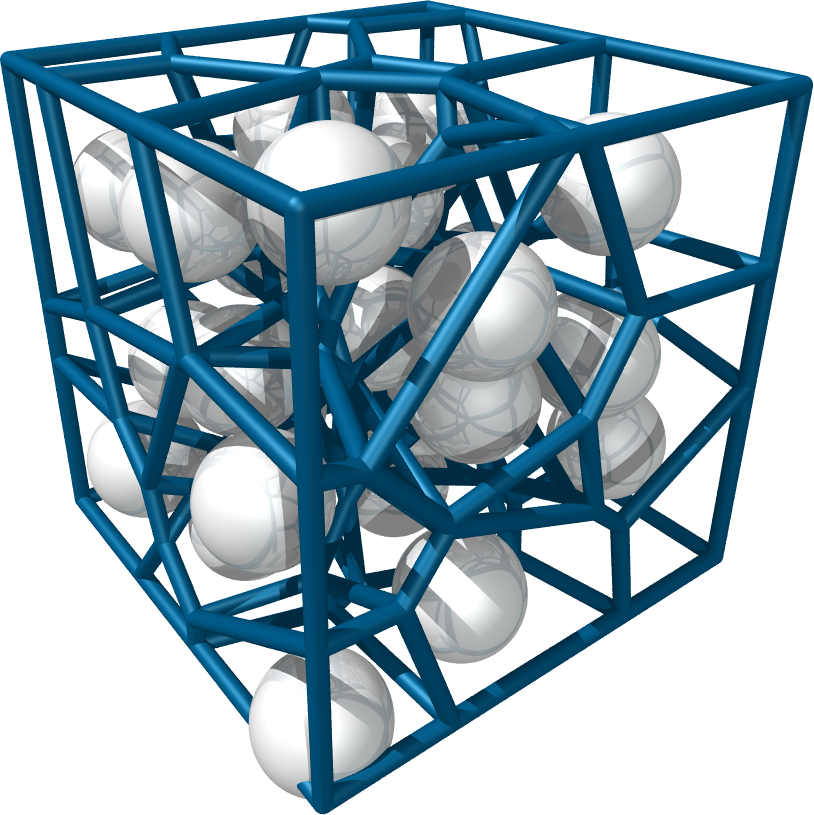
\includegraphics[width=0.8\textwidth]{images/voronoi/3d_diagram04_crop.png}%
        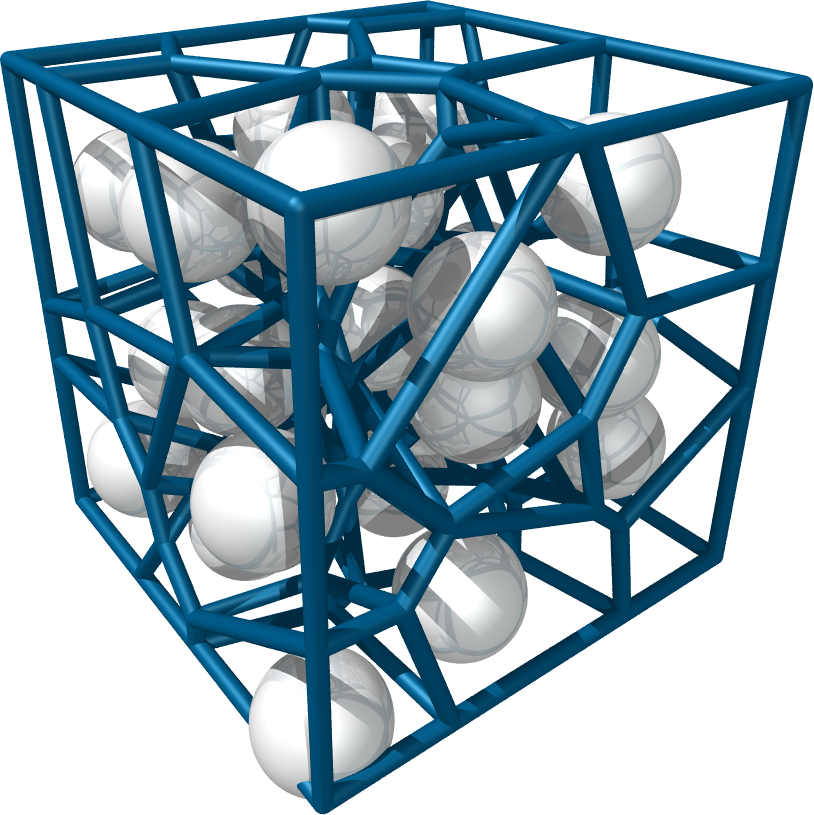
\includegraphics[height=0.7\textwidth]{images/voronoi/3d_diagram04_crop.png}%
        \caption{%
            Rendering of Voronoi cells in 3 dimensions, in a system of 27 particles. Voronoi cells created using the \cpp-library \texttt{Voro++}\cite{rycroft2009voro,webvoro++}, and rendered using the program \texttt{povray}\cite{webpovray}. %
            \label{fig:3d_voronoi_diagram}%
        }%
    \end{minipage}%
\end{figure}%

\todo[inline]{Something about removing hydrogen atoms, and just use oxygen position as hydrogen position, and water atom ``volume''? This simplifies life for us, since we don't have to find which water molecule each hydrogen atom belongs to, but we could get inconsistent water density. But since we use the same method for all measurements, we can compare relative densities.}

\todo[inline]{Something about removing extreme points/tail in distribution? Caused by vacuum.}